
% This LaTeX was auto-generated from MATLAB code.
% To make changes, update the MATLAB code and republish this document.

\documentclass{article}
\usepackage{graphicx}
\usepackage{color}

\sloppy
\definecolor{lightgray}{gray}{0.5}
\setlength{\parindent}{0pt}

\begin{document}

    
    
\subsection*{Contents}

\begin{itemize}
\setlength{\itemsep}{-1ex}
   \item modelagem
   \item Discretização
   \item Requisitos
   \item Controlador 1 - arbitrar zero com o mesmo valor da parte real dos polos desejados
   \item Controlador 2 - utilizando a tática do triângulo isóceles:
   \item Controlador 3 - cancelamento de polo
   \item Análise frequência
   \item Controlador Frequência
\end{itemize}
\begin{verbatim}
close all;
\end{verbatim}


\subsection*{modelagem}

\begin{verbatim}
% captura de resposta ao degrau do carrinho
x(:, 2) = output_real.signals.values;   %posição
x(:, 1) = output_real.time;             %tempo

%Parametros pico e tp
[xm, im] = max(x(:, 2));        %valor de pico
tp = x(im, 1);                  %tepo de pico
xf = mean(x(end-100:end, 2));   %steady-state

%Parametros MP,ksi e wn
Mp = (xm - xf) / xf;                                %overshoot
qsi = log(1 / Mp) / sqrt(pi^2 + (log(1 / Mp))^2);   %fator de amortecimento
wn = pi / (tp * sqrt(1 - qsi^2));                   %frequência natural do sistema
ts2 = 4/(qsi*wn);                                   %tempo de acomodação (2%)

%Parametros a e b
a = 2 * qsi * wn;
b = wn^2;
k = 420 * b; %(xf * wn^2);

%FT em malha aberta
g = tf([b], [1 a 0]);
%FT em malha echada
gs = tf([b], [1 a b]);

% plotting results
plot(x(:,1),x(:,2),'r'); hold on; step(15 *gs, 'b');
title({'Respostas do carrinho e da função de transferência',' obtida à entrada degrau'}); legend ('Carrinho', 'FT - MF');
xlabel('Tempo');

%[REFERÊNCIA]
%<https://www.coursera.org/lecture/controle/formulas-da-resposta-de-segunda-ordem-hIaco>
\end{verbatim}

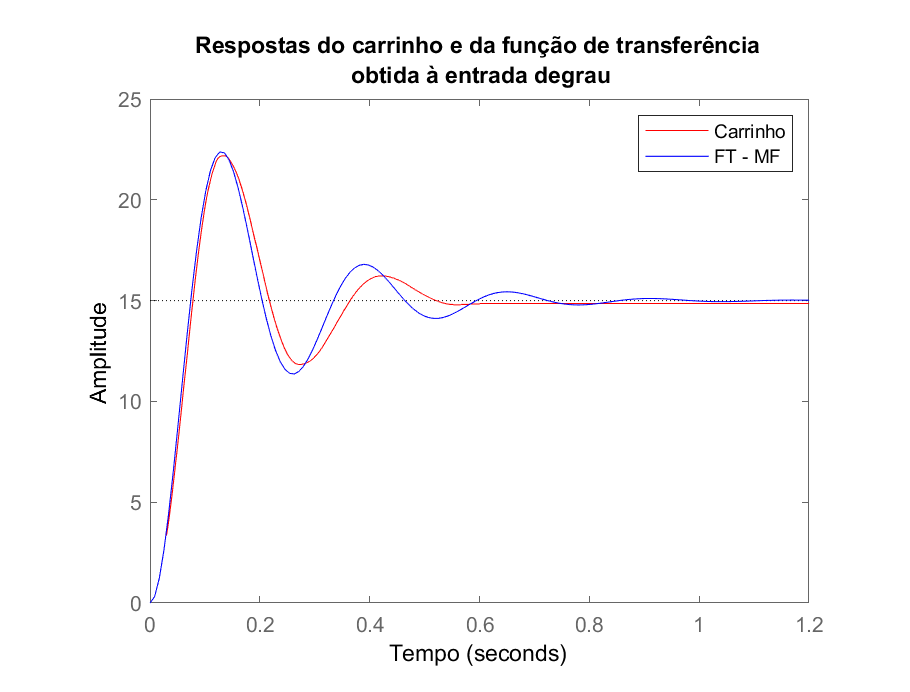
\includegraphics [width=4in]{identifica_01.eps}


\subsection*{Discretização}

\begin{verbatim}
ts = 0.05;                                  %Período de amostragem
discretizado = c2d(g, ts, 'zoh');           %discretizando a FT em malha aberta
[num, den] = tfdata(discretizado, 'v');     %obtendo os vetores de numerador e denominador
polos = roots(den);                         %obtendo o vetor de polos em Z
zeros = roots(num);                         %obtendo o vetor de zeros em Z
\end{verbatim}


\subsection*{Requisitos}

\begin{verbatim}
MPreq = 0.2;            %overshoot máximo de 10%
TS2req = 0.3;           %tempo de acomodação (2%) máximo 0.5s

% Mp = exp ( (- pi * qsi) / sqrt( 1 - qsi^2 ) )
% qsi-req = abs(ln(Mp-req/100))/(sqrt(pi^2+ln(Mp-req/100)^2))
qsi_projeto = ( abs (log(MPreq/100)) / sqrt ((pi^2)+(log(MPreq/100)^2)) );

% Ts2= 4/(qsi*wn)
% wn-req = 4/(qsi-req*Ts2-req)
wn_projeto = 4/ (qsi_projeto * TS2req);

%polo desejado em Z
Zd = exp(-qsi_projeto * wn_projeto * ts) * exp (1j * sqrt(1-(qsi_projeto^2)) * wn_projeto * ts );

figure; rlocus (discretizado); hold on;
scatter (real(Zd),imag(Zd), 'filled');

%[REFERENCIA]
%<https://www.coursera.org/learn/controle-tempo-discreto/lecture/QNGmD/especificacao-de-requisitos-em-tempo-discreto-z-grid>
\end{verbatim}

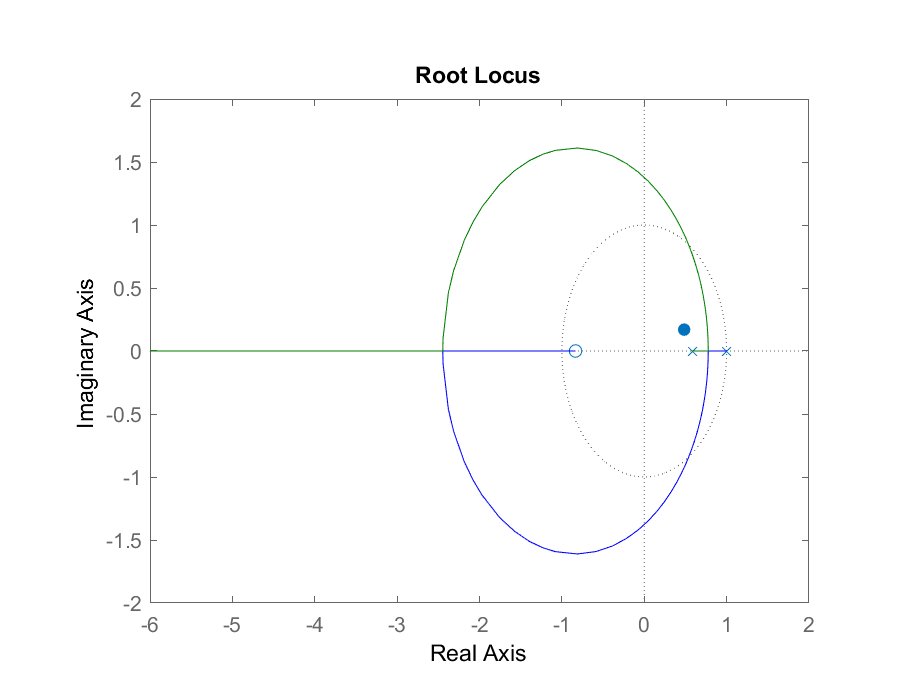
\includegraphics [width=4in]{identifica_02.eps}


\subsection*{Controlador 1 - arbitrar zero com o mesmo valor da parte real dos polos desejados}

\begin{verbatim}
G_Zd = polyval(num, Zd)/polyval(den, Zd);   %valor de G(Z_d)
phaseGZd = phase(G_Zd);                     %radianos
phaseGZddeg = rad2deg (phaseGZd);           %graus

phi = - pi - phaseGZd;              %radianos
phideg = rad2deg(phi);              %graus
phi360 = wrapTo360 (phideg);        %[0º,360º]

% parâmetros
a_proj1 = -real(Zd);
b_proj1 = -real(Zd) + (imag(Zd)*tan((pi/2) - phi));

% ganho
k_proj1 = abs(Zd + b_proj1) / ( abs(Zd + a_proj1)*abs(G_Zd) );

% controlador
Gd1 = zpk (-a_proj1,-b_proj1,k_proj1,ts);

% LGR
figure; rlocus (Gd1 * discretizado); hold on;
scatter (real(Zd),imag(Zd), 'filled');

% step
figure; plot(x(:,1),x(:,2),'r'); hold on; step(15 * gs, 'b'); step (15 * feedback(Gd1*discretizado, 1), 'g'); %step (15-(15*feedback(Gd1*discretizado,1))*Gd1,'y');
title({'Respostas do carrinho, sistema e sistema controlado','à entrada degrau'}); legend ('Carrinho', 'Sistema', 'Sistema controlado');
xlabel('Tempo');

%[REFERÊNCIA]
%<https://www.coursera.org/learn/controle-tempo-discreto/lecture/EgCv7/projeto-de-compensador-de-avanco-de-fase-usando-o-lgr>
\end{verbatim}

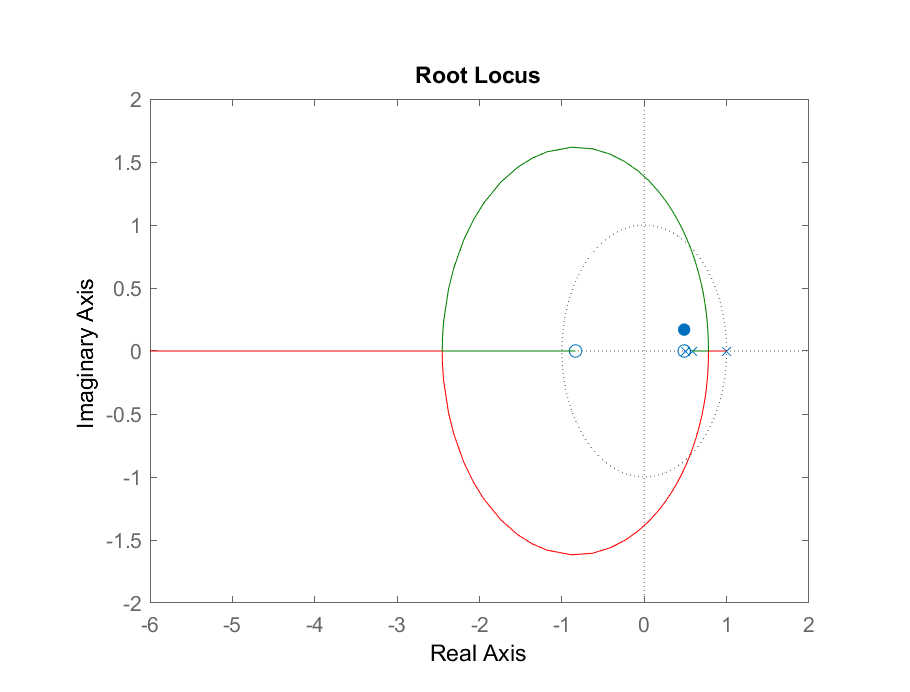
\includegraphics [width=4in]{identifica_03.eps}

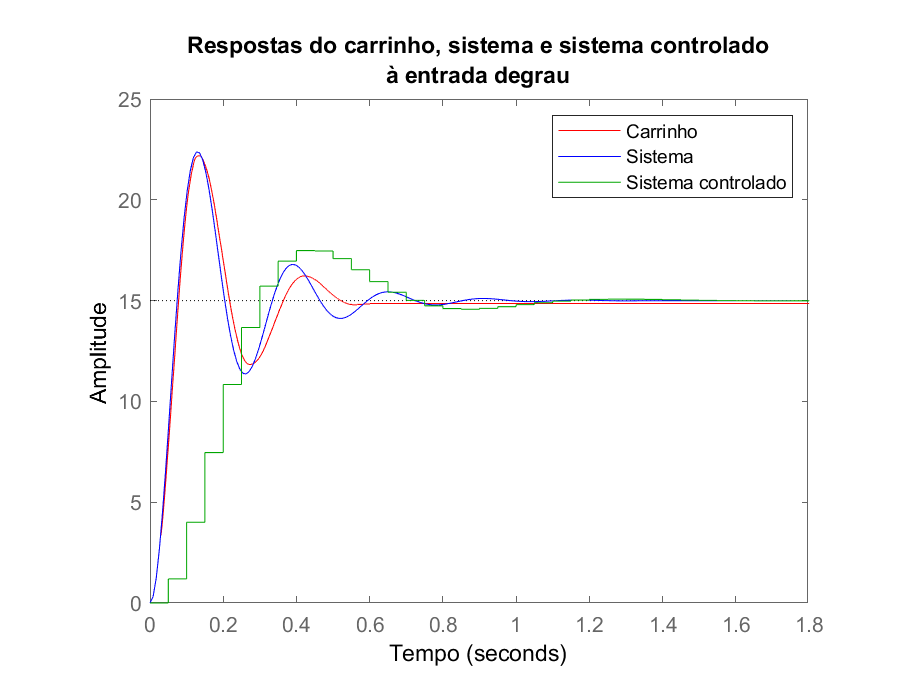
\includegraphics [width=4in]{identifica_04.eps}


\subsection*{Controlador 2 - utilizando a tática do triângulo isóceles:}

\begin{verbatim}
% parâmetros
a_proj2 = - real(Zd) - imag(Zd)*tan((pi/2) - (phi/2));
b_proj2 = - real(Zd) + imag(Zd)*tan((pi/2) - (phi/2));

% ganho
k_proj2 = 1 / abs(G_Zd);

% controlador
Gd2 = zpk (-a_proj2,-b_proj2,k_proj2,ts);

% LGR
figure; rlocus (Gd2 * discretizado); hold on;
scatter (real(Zd),imag(Zd), 'filled');

%step
figure; plot(x(:,1),x(:,2),'r'); hold on; step(15 * gs, 'b'); step (15*feedback(Gd2*discretizado, 1), 'g'); %step (15-(15*feedback(Gd2*discretizado,1))*Gd2,'y');
title({'Respostas do carrinho, sistema e sistema controlado','à entrada degrau'}); legend ('Carrinho', 'Sistema', 'Sistema controlado');
xlabel('Tempo');

%[REFERÊNCIA]
%<https://www.coursera.org/learn/controle-tempo-discreto/lecture/EgCv7/projeto-de-compensador-de-avanco-de-fase-usando-o-lgr>
\end{verbatim}

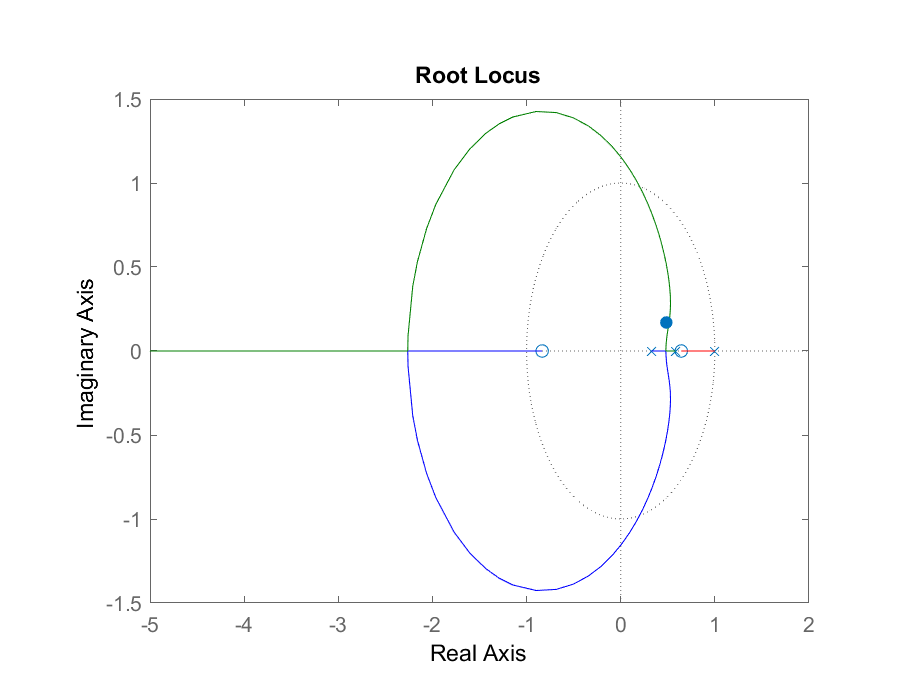
\includegraphics [width=4in]{identifica_05.eps}

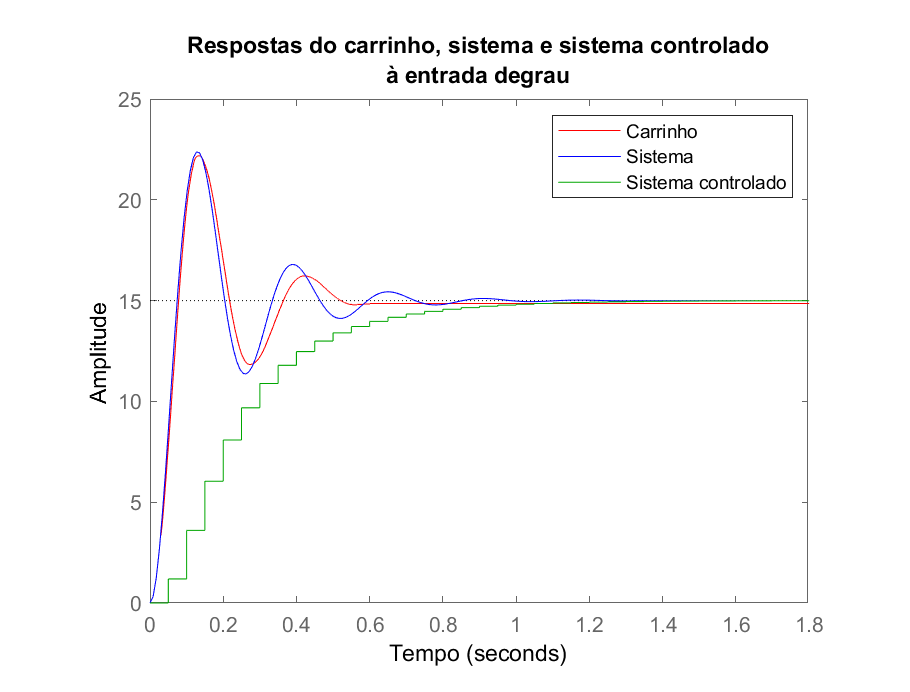
\includegraphics [width=4in]{identifica_06.eps}


\subsection*{Controlador 3 - cancelamento de polo}

\begin{verbatim}
contrib_ang_zero = atan(imag(Zd)/(real(Zd)-zeros(1))); %radianos
contrib_ang_polo1 = atan(imag(Zd)/(real(Zd)-polos(1))); %radianos
contrib_ang_polo2 = atan(imag(Zd)/(real(Zd)-polos(2))); %radianos

soma_das_contrib_ang_em_zd = contrib_ang_zero - contrib_ang_polo1 - contrib_ang_polo2; %radianos
deficiencia_angular = soma_das_contrib_ang_em_zd - pi; %radianos


beta = tan(deficiencia_angular - contrib_ang_polo2)*imag(Zd);
k_gd = abs(Zd + beta) / ( abs(Zd + polos(2))*abs(G_Zd) );
g_d = zpk (polos(2), -beta, k_gd, ts);


% LGR
figure; rlocus (g_d * discretizado); hold on;
scatter (real(Zd),imag(Zd), 'filled');

%step
figure; plot(x(:,1),x(:,2),'r'); hold on; step(15 * gs, 'b'); step (15*feedback(g_d*discretizado, 1), 'g'); %step (15-(15*feedback(Gd2*discretizado,1))*Gd2,'y');
title({'Respostas do carrinho, sistema e sistema controlado','à entrada degrau'}); legend ('Carrinho', 'Sistema', 'Sistema controlado');
xlabel('Tempo');

%[REFERÊNCIA]
%<https://www.coursera.org/learn/controle-tempo-discreto/lecture/EgCv7/projeto-de-compensador-de-avanco-de-fase-usando-o-lgr>
\end{verbatim}

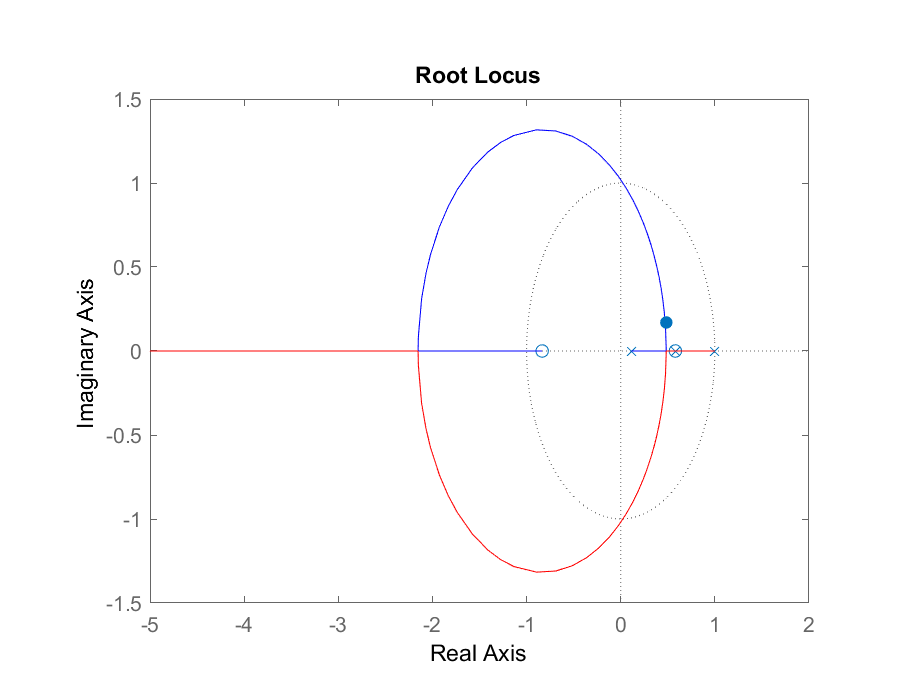
\includegraphics [width=4in]{identifica_07.eps}

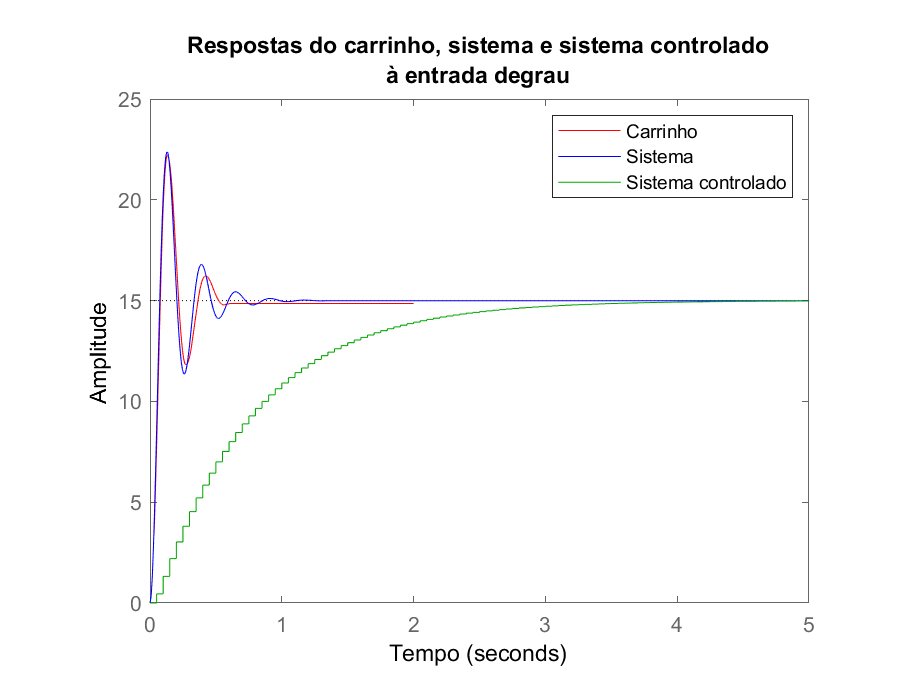
\includegraphics [width=4in]{identifica_08.eps}


\subsection*{Análise frequência}

\begin{verbatim}
[Gm,Pm, Wcg, Wcp] = margin (g);

WnMF = Wcp;
qsiMF = Pm/100;

Mp_freq = exp((-pi*qsiMF)/(sqrt(1-(qsiMF^2))));     % pico
tp_freq = pi/(WnMF*sqrt(1-(qsiMF^2)));              % tempo de pico

% requisitos
MP_req_freq = 0.1;

qsi_proj_freq = abs(log(MP_req_freq))/sqrt((pi^2)+(abs(log(MP_req_freq))^2));
Pm_proj = 100*qsi_proj_freq;



% [REFERENCIA]
% <https://www.coursera.org/learn/controle-tempo-discreto/lecture/Vu9HR/criterios-para-projeto-usando-a-resposta-em-frequencia>
\end{verbatim}


\subsection*{Controlador Frequência}

\begin{verbatim}
%[REFERÊNCIA]
%<https://www.coursera.org/learn/controle-tempo-discreto/lecture/6bKmG/projeto-de-compensador-de-avanco-de-fase-para-atender-sobressinal-e-tempo-de>
\end{verbatim}



\end{document}
    
